% Options for packages loaded elsewhere
% Options for packages loaded elsewhere
\PassOptionsToPackage{unicode}{hyperref}
\PassOptionsToPackage{hyphens}{url}
\PassOptionsToPackage{dvipsnames,svgnames,x11names}{xcolor}
%
\documentclass[
  japanese,
  letterpaper,
]{ltjbook}
\usepackage{xcolor}
\usepackage{amsmath,amssymb}
\setcounter{secnumdepth}{5}
\usepackage{iftex}
\ifPDFTeX
  \usepackage[T1]{fontenc}
  \usepackage[utf8]{inputenc}
  \usepackage{textcomp} % provide euro and other symbols
\else % if luatex or xetex
  \usepackage{unicode-math} % this also loads fontspec
  \defaultfontfeatures{Scale=MatchLowercase}
  \defaultfontfeatures[\rmfamily]{Ligatures=TeX,Scale=1}
\fi
\usepackage{lmodern}
\ifPDFTeX\else
  % xetex/luatex font selection
\fi
% Use upquote if available, for straight quotes in verbatim environments
\IfFileExists{upquote.sty}{\usepackage{upquote}}{}
\IfFileExists{microtype.sty}{% use microtype if available
  \usepackage[]{microtype}
  \UseMicrotypeSet[protrusion]{basicmath} % disable protrusion for tt fonts
}{}
\makeatletter
\@ifundefined{KOMAClassName}{% if non-KOMA class
  \IfFileExists{parskip.sty}{%
    \usepackage{parskip}
  }{% else
    \setlength{\parindent}{0pt}
    \setlength{\parskip}{6pt plus 2pt minus 1pt}}
}{% if KOMA class
  \KOMAoptions{parskip=half}}
\makeatother
% Make \paragraph and \subparagraph free-standing
\makeatletter
\ifx\paragraph\undefined\else
  \let\oldparagraph\paragraph
  \renewcommand{\paragraph}{
    \@ifstar
      \xxxParagraphStar
      \xxxParagraphNoStar
  }
  \newcommand{\xxxParagraphStar}[1]{\oldparagraph*{#1}\mbox{}}
  \newcommand{\xxxParagraphNoStar}[1]{\oldparagraph{#1}\mbox{}}
\fi
\ifx\subparagraph\undefined\else
  \let\oldsubparagraph\subparagraph
  \renewcommand{\subparagraph}{
    \@ifstar
      \xxxSubParagraphStar
      \xxxSubParagraphNoStar
  }
  \newcommand{\xxxSubParagraphStar}[1]{\oldsubparagraph*{#1}\mbox{}}
  \newcommand{\xxxSubParagraphNoStar}[1]{\oldsubparagraph{#1}\mbox{}}
\fi
\makeatother

\usepackage{color}
\usepackage{fancyvrb}
\newcommand{\VerbBar}{|}
\newcommand{\VERB}{\Verb[commandchars=\\\{\}]}
\DefineVerbatimEnvironment{Highlighting}{Verbatim}{commandchars=\\\{\}}
% Add ',fontsize=\small' for more characters per line
\usepackage{framed}
\definecolor{shadecolor}{RGB}{241,243,245}
\newenvironment{Shaded}{\begin{snugshade}}{\end{snugshade}}
\newcommand{\AlertTok}[1]{\textcolor[rgb]{0.68,0.00,0.00}{#1}}
\newcommand{\AnnotationTok}[1]{\textcolor[rgb]{0.37,0.37,0.37}{#1}}
\newcommand{\AttributeTok}[1]{\textcolor[rgb]{0.40,0.45,0.13}{#1}}
\newcommand{\BaseNTok}[1]{\textcolor[rgb]{0.68,0.00,0.00}{#1}}
\newcommand{\BuiltInTok}[1]{\textcolor[rgb]{0.00,0.23,0.31}{#1}}
\newcommand{\CharTok}[1]{\textcolor[rgb]{0.13,0.47,0.30}{#1}}
\newcommand{\CommentTok}[1]{\textcolor[rgb]{0.37,0.37,0.37}{#1}}
\newcommand{\CommentVarTok}[1]{\textcolor[rgb]{0.37,0.37,0.37}{\textit{#1}}}
\newcommand{\ConstantTok}[1]{\textcolor[rgb]{0.56,0.35,0.01}{#1}}
\newcommand{\ControlFlowTok}[1]{\textcolor[rgb]{0.00,0.23,0.31}{\textbf{#1}}}
\newcommand{\DataTypeTok}[1]{\textcolor[rgb]{0.68,0.00,0.00}{#1}}
\newcommand{\DecValTok}[1]{\textcolor[rgb]{0.68,0.00,0.00}{#1}}
\newcommand{\DocumentationTok}[1]{\textcolor[rgb]{0.37,0.37,0.37}{\textit{#1}}}
\newcommand{\ErrorTok}[1]{\textcolor[rgb]{0.68,0.00,0.00}{#1}}
\newcommand{\ExtensionTok}[1]{\textcolor[rgb]{0.00,0.23,0.31}{#1}}
\newcommand{\FloatTok}[1]{\textcolor[rgb]{0.68,0.00,0.00}{#1}}
\newcommand{\FunctionTok}[1]{\textcolor[rgb]{0.28,0.35,0.67}{#1}}
\newcommand{\ImportTok}[1]{\textcolor[rgb]{0.00,0.46,0.62}{#1}}
\newcommand{\InformationTok}[1]{\textcolor[rgb]{0.37,0.37,0.37}{#1}}
\newcommand{\KeywordTok}[1]{\textcolor[rgb]{0.00,0.23,0.31}{\textbf{#1}}}
\newcommand{\NormalTok}[1]{\textcolor[rgb]{0.00,0.23,0.31}{#1}}
\newcommand{\OperatorTok}[1]{\textcolor[rgb]{0.37,0.37,0.37}{#1}}
\newcommand{\OtherTok}[1]{\textcolor[rgb]{0.00,0.23,0.31}{#1}}
\newcommand{\PreprocessorTok}[1]{\textcolor[rgb]{0.68,0.00,0.00}{#1}}
\newcommand{\RegionMarkerTok}[1]{\textcolor[rgb]{0.00,0.23,0.31}{#1}}
\newcommand{\SpecialCharTok}[1]{\textcolor[rgb]{0.37,0.37,0.37}{#1}}
\newcommand{\SpecialStringTok}[1]{\textcolor[rgb]{0.13,0.47,0.30}{#1}}
\newcommand{\StringTok}[1]{\textcolor[rgb]{0.13,0.47,0.30}{#1}}
\newcommand{\VariableTok}[1]{\textcolor[rgb]{0.07,0.07,0.07}{#1}}
\newcommand{\VerbatimStringTok}[1]{\textcolor[rgb]{0.13,0.47,0.30}{#1}}
\newcommand{\WarningTok}[1]{\textcolor[rgb]{0.37,0.37,0.37}{\textit{#1}}}

\usepackage{longtable,booktabs,array}
\usepackage{calc} % for calculating minipage widths
% Correct order of tables after \paragraph or \subparagraph
\usepackage{etoolbox}
\makeatletter
\patchcmd\longtable{\par}{\if@noskipsec\mbox{}\fi\par}{}{}
\makeatother
% Allow footnotes in longtable head/foot
\IfFileExists{footnotehyper.sty}{\usepackage{footnotehyper}}{\usepackage{footnote}}
\makesavenoteenv{longtable}
\usepackage{graphicx}
\makeatletter
\newsavebox\pandoc@box
\newcommand*\pandocbounded[1]{% scales image to fit in text height/width
  \sbox\pandoc@box{#1}%
  \Gscale@div\@tempa{\textheight}{\dimexpr\ht\pandoc@box+\dp\pandoc@box\relax}%
  \Gscale@div\@tempb{\linewidth}{\wd\pandoc@box}%
  \ifdim\@tempb\p@<\@tempa\p@\let\@tempa\@tempb\fi% select the smaller of both
  \ifdim\@tempa\p@<\p@\scalebox{\@tempa}{\usebox\pandoc@box}%
  \else\usebox{\pandoc@box}%
  \fi%
}
% Set default figure placement to htbp
\def\fps@figure{htbp}
\makeatother


% definitions for citeproc citations
\NewDocumentCommand\citeproctext{}{}
\NewDocumentCommand\citeproc{mm}{%
  \begingroup\def\citeproctext{#2}\cite{#1}\endgroup}
\makeatletter
 % allow citations to break across lines
 \let\@cite@ofmt\@firstofone
 % avoid brackets around text for \cite:
 \def\@biblabel#1{}
 \def\@cite#1#2{{#1\if@tempswa , #2\fi}}
\makeatother
\newlength{\cslhangindent}
\setlength{\cslhangindent}{1.5em}
\newlength{\csllabelwidth}
\setlength{\csllabelwidth}{3em}
\newenvironment{CSLReferences}[2] % #1 hanging-indent, #2 entry-spacing
 {\begin{list}{}{%
  \setlength{\itemindent}{0pt}
  \setlength{\leftmargin}{0pt}
  \setlength{\parsep}{0pt}
  % turn on hanging indent if param 1 is 1
  \ifodd #1
   \setlength{\leftmargin}{\cslhangindent}
   \setlength{\itemindent}{-1\cslhangindent}
  \fi
  % set entry spacing
  \setlength{\itemsep}{#2\baselineskip}}}
 {\end{list}}
\usepackage{calc}
\newcommand{\CSLBlock}[1]{\hfill\break\parbox[t]{\linewidth}{\strut\ignorespaces#1\strut}}
\newcommand{\CSLLeftMargin}[1]{\parbox[t]{\csllabelwidth}{\strut#1\strut}}
\newcommand{\CSLRightInline}[1]{\parbox[t]{\linewidth - \csllabelwidth}{\strut#1\strut}}
\newcommand{\CSLIndent}[1]{\hspace{\cslhangindent}#1}

\ifLuaTeX
\usepackage[bidi=basic,provide=*]{babel}
\else
\usepackage[bidi=default,provide=*]{babel}
\fi
% get rid of language-specific shorthands (see #6817):
\let\LanguageShortHands\languageshorthands
\def\languageshorthands#1{}


\setlength{\emergencystretch}{3em} % prevent overfull lines

\providecommand{\tightlist}{%
  \setlength{\itemsep}{0pt}\setlength{\parskip}{0pt}}



 


\makeatletter
\@ifpackageloaded{tcolorbox}{}{\usepackage[skins,breakable]{tcolorbox}}
\@ifpackageloaded{fontawesome5}{}{\usepackage{fontawesome5}}
\definecolor{quarto-callout-color}{HTML}{909090}
\definecolor{quarto-callout-note-color}{HTML}{0758E5}
\definecolor{quarto-callout-important-color}{HTML}{CC1914}
\definecolor{quarto-callout-warning-color}{HTML}{EB9113}
\definecolor{quarto-callout-tip-color}{HTML}{00A047}
\definecolor{quarto-callout-caution-color}{HTML}{FC5300}
\definecolor{quarto-callout-color-frame}{HTML}{acacac}
\definecolor{quarto-callout-note-color-frame}{HTML}{4582ec}
\definecolor{quarto-callout-important-color-frame}{HTML}{d9534f}
\definecolor{quarto-callout-warning-color-frame}{HTML}{f0ad4e}
\definecolor{quarto-callout-tip-color-frame}{HTML}{02b875}
\definecolor{quarto-callout-caution-color-frame}{HTML}{fd7e14}
\makeatother
\makeatletter
\@ifpackageloaded{bookmark}{}{\usepackage{bookmark}}
\makeatother
\makeatletter
\@ifpackageloaded{caption}{}{\usepackage{caption}}
\AtBeginDocument{%
\ifdefined\contentsname
  \renewcommand*\contentsname{目次}
\else
  \newcommand\contentsname{目次}
\fi
\ifdefined\listfigurename
  \renewcommand*\listfigurename{図一覧}
\else
  \newcommand\listfigurename{図一覧}
\fi
\ifdefined\listtablename
  \renewcommand*\listtablename{表一覧}
\else
  \newcommand\listtablename{表一覧}
\fi
\ifdefined\figurename
  \renewcommand*\figurename{図}
\else
  \newcommand\figurename{図}
\fi
\ifdefined\tablename
  \renewcommand*\tablename{表}
\else
  \newcommand\tablename{表}
\fi
}
\@ifpackageloaded{float}{}{\usepackage{float}}
\floatstyle{ruled}
\@ifundefined{c@chapter}{\newfloat{codelisting}{h}{lop}}{\newfloat{codelisting}{h}{lop}[chapter]}
\floatname{codelisting}{コード}
\newcommand*\listoflistings{\listof{codelisting}{コード一覧}}
\usepackage{amsthm}
\theoremstyle{plain}
\newtheorem{theorem}{定理}[chapter]
\theoremstyle{definition}
\newtheorem{example}{例}[chapter]
\theoremstyle{remark}
\AtBeginDocument{\renewcommand*{\proofname}{証明}}
\newtheorem*{remark}{注釈}
\newtheorem*{solution}{解答}
\newtheorem{refremark}{注釈}[chapter]
\newtheorem{refsolution}{解答}[chapter]
\makeatother
\makeatletter
\makeatother
\makeatletter
\@ifpackageloaded{caption}{}{\usepackage{caption}}
\@ifpackageloaded{subcaption}{}{\usepackage{subcaption}}
\makeatother
\usepackage{bookmark}
\IfFileExists{xurl.sty}{\usepackage{xurl}}{} % add URL line breaks if available
\urlstyle{same}
\hypersetup{
  pdftitle={オペレーションズ・リサーチ},
  pdfauthor={劉子昂},
  pdflang={ja},
  colorlinks=true,
  linkcolor={blue},
  filecolor={Maroon},
  citecolor={Blue},
  urlcolor={Blue},
  pdfcreator={LaTeX via pandoc}}


\title{オペレーションズ・リサーチ}
\usepackage{etoolbox}
\makeatletter
\providecommand{\subtitle}[1]{% add subtitle to \maketitle
  \apptocmd{\@title}{\par {\large #1 \par}}{}{}
}
\makeatother
\subtitle{Operations Research: Models, Algorithms, and Implementations}
\author{劉子昂}
\date{2025-09-01}
\begin{document}
\maketitle

\renewcommand*\contentsname{目次}
{
\hypersetup{linkcolor=}
\setcounter{tocdepth}{2}
\tableofcontents
}

\bookmarksetup{startatroot}

\chapter*{Preface}\label{preface}
\addcontentsline{toc}{chapter}{Preface}

\markboth{Preface}{Preface}

This is a Quarto book.

To learn more about Quarto books visit
\url{https://quarto.org/docs/books}.

\part{在庫モデル}

\chapter{在庫管理とは}\label{ux5728ux5eabux7ba1ux7406ux3068ux306f}

商店・工場・倉庫などで、原材料・部品・製品などを適切に管理することを\textbf{在庫管理}(Inventory
Management)という。一般的に、在庫管理の目的は、顧客の需要を満たしつつ、在庫に関わる費用を最小化することである。

\begin{tcolorbox}[enhanced jigsaw, colbacktitle=quarto-callout-note-color!10!white, breakable, opacitybacktitle=0.6, bottomrule=.15mm, title=\textcolor{quarto-callout-note-color}{\faInfo}\hspace{0.5em}{ノート}, leftrule=.75mm, toprule=.15mm, titlerule=0mm, colback=white, colframe=quarto-callout-note-color-frame, bottomtitle=1mm, toptitle=1mm, arc=.35mm, rightrule=.15mm, opacityback=0, left=2mm, coltitle=black]

豊田自動車が提唱した\textbf{ジャストインタイム}(Just In Time,
JIT)は、生産方式としてよく知られている。

JIT とは必要なものを、必要な時に、必要な量だけ生産することである。JIT
の目的は、在庫を最小限に抑え、効率的な生産を実現することである。

アメリカの研究者らは、その生産方式を体系化し、\textbf{リーン生産方式}(Lean
Manufacturing)という概念を提唱した。

\begin{itemize}
\tightlist
\item
  \href{https://global.toyota/jp/company/vision-and-philosophy/production-system/}{トヨタ生産方式}
\end{itemize}

\end{tcolorbox}

在庫が多すぎると、保管費用がかかる。逆に、在庫が少なすぎると、欠品が発生し、顧客の需要を満たせなくなる。在庫管理は次の二つの問題を決定する。

\begin{enumerate}
\def\labelenumi{\arabic{enumi}.}
\tightlist
\item
  どのくらいの量を発注するか?(発注量)
\item
  いつ発注するか?(発注時期)
\end{enumerate}

科学的在庫管理(Scientific Inventory
Management)では、これらの問題に答えるために、次の手順で在庫管理を行う。

\begin{enumerate}
\def\labelenumi{\arabic{enumi}.}
\tightlist
\item
  在庫システムを数学モデルとして定式化する。
\item
  最適な発注量と発注時期を決定する。
\end{enumerate}

\section{在庫モデルの分類}\label{ux5728ux5eabux30e2ux30c7ux30ebux306eux5206ux985e}

在庫モデルは、次のような要素で分類される。

\begin{description}
\tightlist
\item[需要(demand)]
需要が決定論的 (Deterministic) か確率的(Stochastic)か。
\item[観測(review)]
在庫量を連続観測 (Continuous Review) するか、周期観測 (Periodic Review)
するか。連続観測の場合、在庫量が連続的に観測でき、いつでも発注が可能である。周期観測の場合、一定の期間(例えば1週間)ごとに在庫量を観測する。
\item[リードタイム(lead time)]
発注から納品までの期間。調達期間とも呼ばれる。リードタイムが決定論的か確率的か。また、リードタイムが0かどうか。在庫モデルを単純化するために、リードタイムを0とし、発注から納品までの期間を無視することもある。
\item[バックオーダー(backorder)]
バックオーダーが許容されるかどうか。需要が在庫を上回った場合、バックオーダーが許容されると、欠品が発生しても、後で需要を満たすことができる。バックオーダーが許容されない場合、欠品が発生すると、上回った需要は失われ、機会損失が発生する。
\item[計画期間(planning horizon)]
単一期間 (Single Period) か、複数期間 (Multi Period) か、無限 (Infinite)
か。
\end{description}

以下の表に、需要と観測に基づく、古典的な在庫モデルを示す。

\begin{longtable}[]{@{}lll@{}}
\toprule\noalign{}
在庫モデル & 需要 & 観測 \\
\midrule\noalign{}
\endhead
\bottomrule\noalign{}
\endlastfoot
EOQモデル & 決定論的 & 連続観測 \\
Wagner-Whitin & 決定論的 & 周期観測 \\
安全在庫 & 確率的 & 連続観測 \\
新聞売り子問題 & 確率的 & 周期観測 \\
\end{longtable}

\section{在庫の費用}\label{ux5728ux5eabux306eux8cbbux7528}

ここでは、在庫に関わる費用を紹介する。

\begin{description}
\tightlist
\item[発注費用(ordering cost)]
発注量に関わらず、1回の発注にかかる費用。調達費用、固定費用(fixed
cost)などとも呼ばれる。通常、1回の発注にかかる費用を \(K\) とする。
\item[購入費用(purchase cost)]
商品を購入するためにかかる費用。通常、単位あたりの購入費用を \(c\)
とする。
\item[欠品費用(stockout cost)]
需要が在庫を上回った場合に発生する費用。通常、単位あたりの欠品費用を
\(p\) とする。
\item[保管費用(holding cost)]
在庫を保管するためにかかる倉庫費用、保険費用、税金、機会費用など。通常、単位時間あたりの1単位あたりの保管費用を
\(h\) とする。
\end{description}

例えば、1日あたり1単位の在庫を保管するために、\(h\)
の費用がかかるとする。30日間、50単位の在庫を保管するための総保管費用は
\(30 \times 50 \times h = 1500h\) となる。下の図を見ると、保管費用は

\[
\text{面積} \times h = 1500h
\]

となることがわかる。

\begin{Shaded}
\begin{Highlighting}[]
\ImportTok{import}\NormalTok{ matplotlib.pyplot }\ImportTok{as}\NormalTok{ plt}
\ImportTok{import}\NormalTok{ numpy }\ImportTok{as}\NormalTok{ np}

\NormalTok{t }\OperatorTok{=}\NormalTok{ np.linspace(}\DecValTok{0}\NormalTok{, }\DecValTok{30}\NormalTok{, }\DecValTok{1000}\NormalTok{)}
\NormalTok{inventory }\OperatorTok{=}\NormalTok{ np.full\_like(t, }\DecValTok{50}\NormalTok{)}

\CommentTok{\# Plotting the inventory level}
\NormalTok{plt.fill\_between(t, inventory, color}\OperatorTok{=}\StringTok{"lightgray"}\NormalTok{, alpha}\OperatorTok{=}\FloatTok{0.5}\NormalTok{, label}\OperatorTok{=}\StringTok{"Inventory Level"}\NormalTok{)}
\NormalTok{plt.plot(t, inventory, label}\OperatorTok{=}\StringTok{"Inventory Level"}\NormalTok{, color}\OperatorTok{=}\StringTok{"black"}\NormalTok{, linewidth}\OperatorTok{=}\DecValTok{2}\NormalTok{)}
\NormalTok{plt.xlabel(}\StringTok{"Time"}\NormalTok{)}
\NormalTok{plt.ylabel(}\StringTok{"Inventory Level"}\NormalTok{)}
\NormalTok{plt.axhline(}\DecValTok{0}\NormalTok{, color}\OperatorTok{=}\StringTok{"gray"}\NormalTok{, linewidth}\OperatorTok{=}\DecValTok{1}\NormalTok{)}
\NormalTok{plt.tight\_layout()}
\NormalTok{plt.show()}
\end{Highlighting}
\end{Shaded}

\pandocbounded{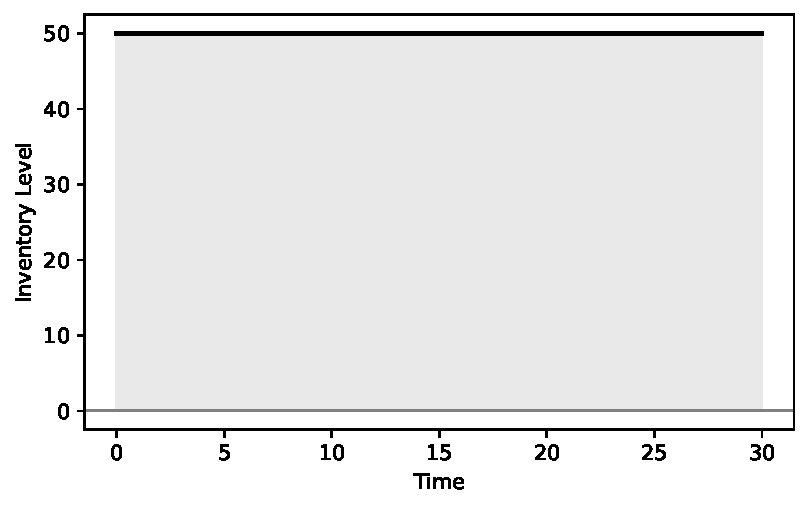
\includegraphics[keepaspectratio]{inventory/intro_files/figure-pdf/cell-2-output-1.pdf}}

一般的に、在庫量が定数ではなく、時間とともに変化する。例えば、発注量を
\(500\) とし、6 日間の在庫量を考える。

\begin{Shaded}
\begin{Highlighting}[]
\CommentTok{\# Parameters}
\NormalTok{d }\OperatorTok{=} \DecValTok{250}  \CommentTok{\# Demand rate}
\NormalTok{Q }\OperatorTok{=} \DecValTok{500}  \CommentTok{\# Order quantity}
\NormalTok{T }\OperatorTok{=}\NormalTok{ Q }\OperatorTok{/}\NormalTok{ d  }\CommentTok{\# Cycle length}
\NormalTok{t }\OperatorTok{=}\NormalTok{ np.linspace(}\DecValTok{0}\NormalTok{, }\FloatTok{2.999} \OperatorTok{*}\NormalTok{ T, }\DecValTok{1000}\NormalTok{)}

\CommentTok{\# Inventory level over time}
\NormalTok{inventory }\OperatorTok{=}\NormalTok{ np.maximum(}\DecValTok{0}\NormalTok{, Q }\OperatorTok{{-}}\NormalTok{ (d }\OperatorTok{*}\NormalTok{ t) }\OperatorTok{\%}\NormalTok{ Q)}

\CommentTok{\# Plotting the inventory level}
\NormalTok{plt.fill\_between(t, inventory, color}\OperatorTok{=}\StringTok{"lightgray"}\NormalTok{, alpha}\OperatorTok{=}\FloatTok{0.5}\NormalTok{, label}\OperatorTok{=}\StringTok{"Inventory Level"}\NormalTok{)}
\NormalTok{plt.plot(t, inventory, label}\OperatorTok{=}\StringTok{"Inventory Level"}\NormalTok{, color}\OperatorTok{=}\StringTok{"black"}\NormalTok{, linewidth}\OperatorTok{=}\DecValTok{2}\NormalTok{)}
\NormalTok{plt.xlabel(}\StringTok{"Time"}\NormalTok{)}
\NormalTok{plt.ylabel(}\StringTok{"Inventory Level"}\NormalTok{)}
\NormalTok{plt.axhline(}\DecValTok{0}\NormalTok{, color}\OperatorTok{=}\StringTok{"gray"}\NormalTok{, linewidth}\OperatorTok{=}\DecValTok{1}\NormalTok{)}
\NormalTok{plt.ylim(bottom}\OperatorTok{=}\DecValTok{0}\NormalTok{, top}\OperatorTok{=}\NormalTok{Q }\OperatorTok{+} \DecValTok{200}\NormalTok{)}
\NormalTok{plt.tight\_layout()}
\NormalTok{plt.show()}
\end{Highlighting}
\end{Shaded}

\pandocbounded{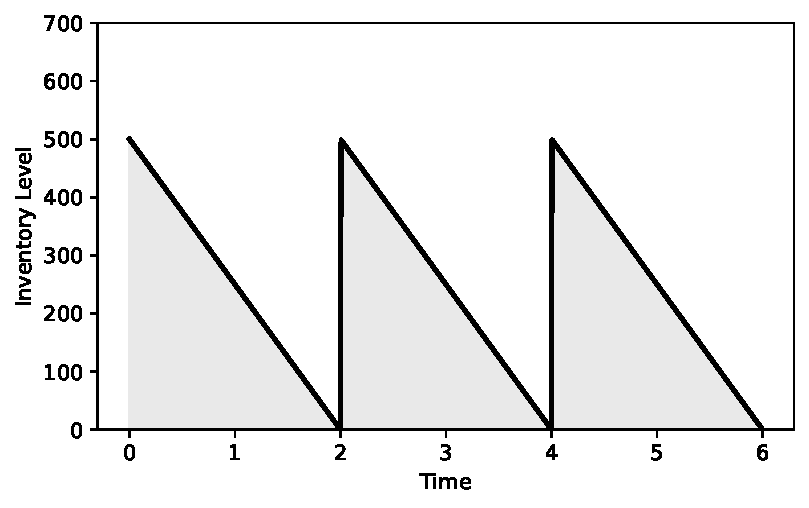
\includegraphics[keepaspectratio]{inventory/intro_files/figure-pdf/cell-3-output-1.pdf}}

保管費用は次のように計算される。

\[
\frac{2 \times 500}{2} \times 3 \times h
\]

\chapter{経済的発注量}\label{ux7d4cux6e08ux7684ux767aux6ce8ux91cf}

\textbf{経済的発注量}(EOQ: Economic Order
Quantity)モデルは、最も基本的な在庫管理モデルの一つである。Harris
(1990) このモデルを最初に提案した。

EOQモデルは、単位時間あたりの需要量は決定論的で、一定であると仮定する。すなわち、需要量は事前に分かっており、時間とともに変化しない。単位時間あたりの需要量は需要率(demand
rate)と呼ばれ、記号 \(d\)
で表される。リードタイムは0とし、発注から納品までの時間はないと仮定する。一回の発注量を
\(Q\)
とし、一定であるとする。欠品は許せないとする。全ての需要は満されなければならない。また、EOQモデルでは、在庫量は連続的に観測され、いつでも発注が可能であるとする。

在庫に関わる費用は、発注費用 \(K\)、保管費用 \(h\)
と、購入費用(購入単価を \(c\) と表す)がある。

EOQモデルの最適解は次の二つの性質を持つ(Snyder と Shen 2019):

\begin{enumerate}
\def\labelenumi{\arabic{enumi}.}
\tightlist
\item
  Zero-inventory ordering (ZIO).
  在庫量が0のときに発注を行う。リードタイムは0であるため、在庫量が0でないときに発注すると、保管費用が発生する。
\item
  Constant order sizes. 発注量は一定である。需要率 \(d\)
  が一定であり、在庫量が0のときに発注を行うため、最適発注量も一定である。
\end{enumerate}

以上の性質から、在庫量の時間的変化は下図のようになる。

\begin{Shaded}
\begin{Highlighting}[]
\ImportTok{import}\NormalTok{ matplotlib.pyplot }\ImportTok{as}\NormalTok{ plt}
\ImportTok{import}\NormalTok{ numpy }\ImportTok{as}\NormalTok{ np}

\CommentTok{\# Parameters}
\NormalTok{d }\OperatorTok{=} \DecValTok{250}  \CommentTok{\# Demand rate}
\NormalTok{Q }\OperatorTok{=} \DecValTok{500}  \CommentTok{\# Order quantity}
\NormalTok{T }\OperatorTok{=}\NormalTok{ Q }\OperatorTok{/}\NormalTok{ d  }\CommentTok{\# Cycle length}
\NormalTok{t }\OperatorTok{=}\NormalTok{ np.linspace(}\DecValTok{0}\NormalTok{, }\DecValTok{3} \OperatorTok{*}\NormalTok{ T, }\DecValTok{1000}\NormalTok{)  }\CommentTok{\# Time from 0 to 3 cycles}

\CommentTok{\# Inventory level over time}
\NormalTok{inventory }\OperatorTok{=}\NormalTok{ np.maximum(}\DecValTok{0}\NormalTok{, Q }\OperatorTok{{-}}\NormalTok{ (d }\OperatorTok{*}\NormalTok{ t) }\OperatorTok{\%}\NormalTok{ Q)}
\NormalTok{inventory[}\DecValTok{0}\NormalTok{] }\OperatorTok{=} \DecValTok{0}

\CommentTok{\# Plotting the inventory level}
\NormalTok{plt.plot(t, inventory, label}\OperatorTok{=}\StringTok{"Inventory Level"}\NormalTok{, color}\OperatorTok{=}\StringTok{"black"}\NormalTok{, linewidth}\OperatorTok{=}\DecValTok{2}\NormalTok{)}
\NormalTok{plt.xlabel(}\StringTok{"Time"}\NormalTok{)}
\NormalTok{plt.ylabel(}\StringTok{"Inventory Level"}\NormalTok{)}
\NormalTok{plt.axhline(}\DecValTok{0}\NormalTok{, color}\OperatorTok{=}\StringTok{"gray"}\NormalTok{, linewidth}\OperatorTok{=}\DecValTok{1}\NormalTok{)}
\NormalTok{plt.ylim(bottom}\OperatorTok{=}\DecValTok{0}\NormalTok{, top}\OperatorTok{=}\NormalTok{Q }\OperatorTok{+} \DecValTok{100}\NormalTok{)}
\NormalTok{plt.tight\_layout()}
\NormalTok{plt.show()}
\end{Highlighting}
\end{Shaded}

\pandocbounded{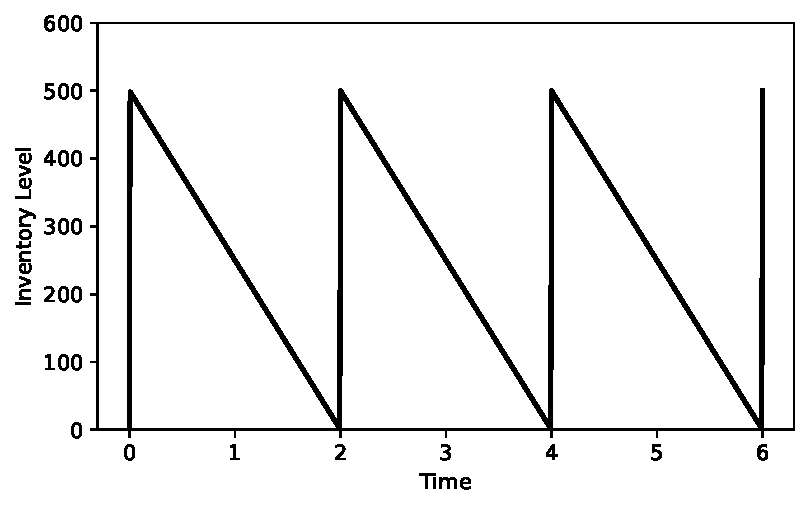
\includegraphics[keepaspectratio]{inventory/eoq_files/figure-pdf/cell-2-output-1.pdf}}

発注の間隔を\textbf{サイクル}(cycle)と呼び、サイクル期間は

\[
T = \frac{Q}{d}
\]

で与えられる。

\begin{example}[]\protect\hypertarget{exm-cycle}{}\label{exm-cycle}

A社は、毎月250個の需要がある商品を取り扱っている。一回の発注量は500個とし、サイクル期間は

\[
T = \frac{500}{250} = 2 \text{ヶ月}
\]

となる。

\end{example}

\section{コスト関数}\label{ux30b3ux30b9ux30c8ux95a2ux6570}

ここでは、1サイクルあたりのコストを考える。

\textbf{発注費用}:発注は1回だけ行うため、発注費用は \(K\) である。

\textbf{購入費用}:\(Q\) 個の商品を単価 \(c\) で購入するため、購入費用は
\(cQ\) である。

\textbf{保管費用}:在庫量はサイクル期間 \(T\) の間に \(Q\)
個から0個まで減少するため、平均在庫量は \(\frac{Q}{2}\)
である。したがって、平均保管費用は \(\frac{hQ}{2}\) である。サイクル期間
\(T\) は \(\frac{Q}{d}\) であるため、1サイクルあたりの保管費用は

\[
\frac{hQ}{2} \cdot T = \frac{hQ^2}{2d}
\]

となる。

以上より、1サイクルあたりのコストは次のように表される。

\[
K + cQ + \frac{hQ^2}{2d}
\]

平均コストは、これをサイクル期間 \(T\)
で割ったものとして定義される。したがって、平均コスト \(g(Q)\)
は次のように表される。

\begin{align*}
g(Q) &= \frac{1}{T} \left( K + cQ + \frac{hQ^2}{2d} \right) \\
&= \frac{d}{Q} \left( K + cQ + \frac{hQ^2}{2d} \right) \\
&= \frac{Kd}{Q} + c d + \frac{hQ}{2}
\end{align*}

以上より、平均コストは発注量 \(Q\) の関数として次のように表される。

\[
g(Q) = \frac{Kd}{Q} + cd + \frac{hQ}{2}
\]

\section{最適発注量}\label{ux6700ux9069ux767aux6ce8ux91cf}

EOQモデルの目的は、平均コスト \(g(Q)\) を最小化する発注量 \(Q\)
を求めることである。

平均コストの導関数 \(g'(Q)\) が 0 となる点を求めることで、最適発注量
\(Q^*\) を求めることができる。

\[
g'(Q) = -\frac{Kd}{Q^2} + \frac{h}{2} = 0
\]

これを解くと、最適発注量

\[
Q^* = \sqrt{\frac{2Kd}{h}}
\]

を得る。これをEOQ公式(EOQ formula)と呼ぶ。\(Q^*\)
を経済的発注量と呼ぶ(経済的は最適という意味である)。

二階導関数 \(g''(Q)\)
を求めて、最適発注量が最小値を与えることを確認する。

\[
g''(Q) = \frac{2Kd}{Q^3} > 0
\]

\(g''(Q) > 0\) であるため、\(Q^*\) は最小値を与える。

最適発注量 \(Q^*\) を次の定理にまとめる。

\begin{theorem}[]\protect\hypertarget{thm-eoq}{}\label{thm-eoq}

EOQモデルにおいて、最適発注量 \(Q^*\) は \[
Q^* = \sqrt{\frac{2Kd}{h}}
\]

で与えられる。

\end{theorem}

\(Q^*\) を用いて、最適なサイクル期間 \(T^*\) を求めることができる。

\[
T^* = \frac{Q^*}{d} = \sqrt{\frac{2K}{hd}}
\]

\begin{refremark}
以下の性質がわかる。

\begin{enumerate}
\def\labelenumi{\arabic{enumi}.}
\tightlist
\item
  \(Q^*\) は \(c\) には依存しない。
\item
  \(h\) の増加に伴い、\(Q^*\)
  は減少する。保管費用が高い場合は、少量で高い頻度で発注することが望ましい。
\item
  \(K\) の増加に伴い、\(Q^*\)
  は増加する。発注費用が高い場合は、多量で低い頻度で発注することが望ましい。
\end{enumerate}

\label{rem-eoq-properties}

\end{refremark}

次の図は、発注コスト、保管コスト、平均コストの関係を示している。購入単価を
\(c = 0\) とする。

\begin{Shaded}
\begin{Highlighting}[]
\CommentTok{\# Parameters}
\NormalTok{K }\OperatorTok{=} \DecValTok{500}  \CommentTok{\# Order cost}
\NormalTok{h }\OperatorTok{=} \DecValTok{15}  \CommentTok{\# Holding cost}
\NormalTok{c }\OperatorTok{=} \DecValTok{0}  \CommentTok{\# Purchase cost}
\NormalTok{Q }\OperatorTok{=}\NormalTok{ np.linspace(}\DecValTok{1}\NormalTok{, }\DecValTok{50}\NormalTok{, }\DecValTok{50}\NormalTok{)}

\CommentTok{\# Average cost function}
\NormalTok{g }\OperatorTok{=}\NormalTok{ (K }\OperatorTok{/}\NormalTok{ Q) }\OperatorTok{+}\NormalTok{ c }\OperatorTok{+}\NormalTok{ (h }\OperatorTok{*}\NormalTok{ Q }\OperatorTok{/} \DecValTok{2}\NormalTok{)}

\CommentTok{\# Plotting the costs vs order quantity}
\NormalTok{plt.plot(Q, K }\OperatorTok{/}\NormalTok{ Q, label}\OperatorTok{=}\StringTok{"Order Cost"}\NormalTok{, color}\OperatorTok{=}\StringTok{"blue"}\NormalTok{, linewidth}\OperatorTok{=}\DecValTok{2}\NormalTok{)}
\NormalTok{plt.plot(Q, c }\OperatorTok{+}\NormalTok{ (h }\OperatorTok{*}\NormalTok{ Q }\OperatorTok{/} \DecValTok{2}\NormalTok{), label}\OperatorTok{=}\StringTok{"Holding Cost"}\NormalTok{, color}\OperatorTok{=}\StringTok{"orange"}\NormalTok{, linewidth}\OperatorTok{=}\DecValTok{2}\NormalTok{)}
\NormalTok{plt.plot(Q, g, label}\OperatorTok{=}\StringTok{"Average Cost"}\NormalTok{, color}\OperatorTok{=}\StringTok{"green"}\NormalTok{, linewidth}\OperatorTok{=}\DecValTok{2}\NormalTok{)}
\NormalTok{plt.axvline(}
\NormalTok{    x}\OperatorTok{=}\NormalTok{np.sqrt(}\DecValTok{2} \OperatorTok{*}\NormalTok{ K }\OperatorTok{/}\NormalTok{ h),}
\NormalTok{    color}\OperatorTok{=}\StringTok{"red"}\NormalTok{,}
\NormalTok{    linestyle}\OperatorTok{=}\StringTok{"{-}{-}"}\NormalTok{,}
\NormalTok{    label}\OperatorTok{=}\StringTok{"Optimal Order Quantity"}\NormalTok{,}
\NormalTok{    linewidth}\OperatorTok{=}\DecValTok{2}\NormalTok{,}
\NormalTok{)}
\NormalTok{plt.xlabel(}\StringTok{"Order Quantity (Q)"}\NormalTok{)}
\NormalTok{plt.ylabel(}\StringTok{"Cost"}\NormalTok{)}
\NormalTok{plt.tight\_layout()}
\NormalTok{plt.show()  }
\end{Highlighting}
\end{Shaded}

\pandocbounded{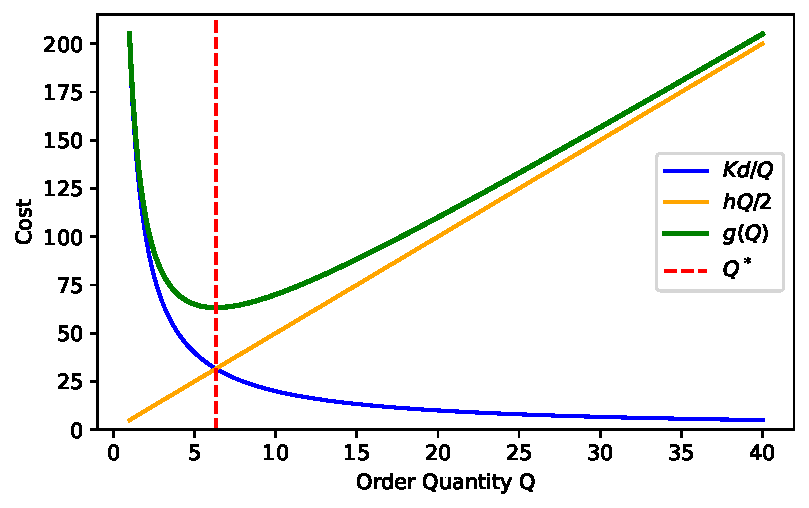
\includegraphics[keepaspectratio]{inventory/eoq_files/figure-pdf/cell-3-output-1.pdf}}

平均コストが最小となる発注量 \(Q^*\)
は、発注コストと保管コストの交差点である。すなわち、発注コストと保管コストを等しくする発注量は最適な発注量
\(Q^*\) である。この性質は以下の式からわかる。

\[
\frac{Kd}{Q^*} = \frac{hQ^*}{2} \Longrightarrow Q^* = \sqrt{\frac{2Kd}{h}}
\]

また、この図からもわかるように、\(Q\)
の増加に伴い、平均発注コストは減少し、平均保管コストは増加する。逆もまた然りである。

\begin{example}[]\protect\hypertarget{exm-eoq}{}\label{exm-eoq}

ある電気量販店では、毎月250台のPCが販売されている。発注費用は5000円、保管費用は1台あたり月150円、購入単価は10万円とする。このとき、最適発注量
\(Q^*\) は次のように求められる。

\[
Q^* = \sqrt{\frac{2 \cdot 5000 \cdot 250}{150}}
\]

最適発注量 \(Q^*\) を次で計算する。

\begin{Shaded}
\begin{Highlighting}[]
\KeywordTok{def}\NormalTok{ eoq(K, d, h):}
    \CommentTok{"""}
\CommentTok{    Calculate the Economic Order Quantity (EOQ).}

\CommentTok{    Parameters:}
\CommentTok{    K (float): Order cost}
\CommentTok{    d (float): Demand rate}
\CommentTok{    h (float): Holding cost}

\CommentTok{    Returns:}
\CommentTok{    float: Optimal order quantity Q*}
\CommentTok{    """}
    \ControlFlowTok{return}\NormalTok{ np.sqrt(}\DecValTok{2} \OperatorTok{*}\NormalTok{ K }\OperatorTok{*}\NormalTok{ d }\OperatorTok{/}\NormalTok{ h)}


\ControlFlowTok{if} \VariableTok{\_\_name\_\_} \OperatorTok{==} \StringTok{"\_\_main\_\_"}\NormalTok{:}
\NormalTok{    K }\OperatorTok{=} \DecValTok{5000}  \CommentTok{\# Order cost}
\NormalTok{    d }\OperatorTok{=} \DecValTok{250}  \CommentTok{\# Demand rate (units per month)}
\NormalTok{    h }\OperatorTok{=} \DecValTok{150}  \CommentTok{\# Holding cost (per unit per month)}

\NormalTok{    Q\_star }\OperatorTok{=}\NormalTok{ eoq(K, d, h)}
    \BuiltInTok{print}\NormalTok{(}\SpecialStringTok{f"Optimal Order Quantity (Q*): }\SpecialCharTok{\{}\NormalTok{Q\_star}\SpecialCharTok{:.2f\}}\SpecialStringTok{"}\NormalTok{)}
\end{Highlighting}
\end{Shaded}

\begin{verbatim}
Optimal Order Quantity (Q*): 129.10
\end{verbatim}

PCの場合は、注文量が整数である必要があるため、\(g(129)\) と \(g(130)\)
を比較して最適発注量を決定する。

\end{example}

\section{リードタイム}\label{ux30eaux30fcux30c9ux30bfux30a4ux30e0}

EOQ モデルでは、リードタイムは0と仮定している。リードタイムが \(L > 0\)
の場合も、最適発注量 \(Q^*\) も変換せず、\(L\) 期間前に \(Q^*\)
を発注すればよい。

ここでは、\(r\) を発注点(reorder point)とする。在庫量が \(r\)
になったときに発注を行う。リードタイム \(L\) の間に需要が \(dL\)
個あるため、発注点は次のように表される。

\[
r = dL
\]

\begin{example}[]\protect\hypertarget{exm-reorder-point}{}\label{exm-reorder-point}

上の例で、リードタイムが一週間とし、一か月を4週間とすると、リードタイムは
\(L = 1/4\) となる。したがって、発注点は次のように求められる。

\[
r = dL = 250 \times \frac{1}{4} = 62.5
\]

PCの在庫量が63台になったときに発注を行う。

\end{example}

\section{他のEOQモデル}\label{ux4ed6ux306eeoqux30e2ux30c7ux30eb}

\begin{itemize}
\tightlist
\item
  バックオーダーを考慮したEOQモデル
\item
  数量割引(quantity discount)を考慮したEOQモデル

  \begin{itemize}
  \tightlist
  \item
    総量割引(all-units discount)
  \item
    増分割引(incremental discount)
  \end{itemize}
\end{itemize}

\chapter{新聞売り子問題}\label{ux65b0ux805eux58f2ux308aux5b50ux554fux984c}

新聞売り子問題(Newsvendor
Problem)は、古典的な確率的在庫モデルの一つである。新聞は次の日には売れなくなるため、新聞売り子問題は最も単純な
perishable 在庫モデルとして知られている。

新聞売り子が新聞を仕入れ、販売する問題を考える。新聞 1 部の仕入れ価格を
\(c\)、販売価格を \(r\)、残存価額を \(v\)、欠品費用を \(p\)、保管費用を
\(h\) とする。ここで、以下の条件を満たすとする。

\begin{itemize}
\tightlist
\item
  \(r > c\). 販売価格は仕入れ価格より高い。
\item
  \(r > v\). 販売価格は残存価値より高い。
\end{itemize}

また、初期在庫は 0 であると仮定する。

新聞の需要 \(D\) は正規分布 \(N(\mu, \sigma^2)\) に従い、\(\mu\) と
\(\sigma\)
は既知である。新聞売り子はどれだけの新聞を発注すればよいかという問題である。

\section{定式化}\label{ux5b9aux5f0fux5316}

ある日、新聞売り子が \(S\) 部の新聞を仕入れ、需要 \(D\) が \(d\)
であったとする。このとき、新聞売り子の利益は以下のように表される。

\[
\pi(S, d) = r \min\{d, S\} - cS + v \max\{0, S - d\} \\
- h \max\{0, S - d\} - p \max\{0, d - S\}
\]

第一項は販売利益、第二項は仕入れコスト、第三項は残存価値、第四項は保管コスト、第五項は欠品コストである。

\begin{tcolorbox}[enhanced jigsaw, colbacktitle=quarto-callout-note-color!10!white, breakable, opacitybacktitle=0.6, bottomrule=.15mm, title=\textcolor{quarto-callout-note-color}{\faInfo}\hspace{0.5em}{ノート}, leftrule=.75mm, toprule=.15mm, titlerule=0mm, colback=white, colframe=quarto-callout-note-color-frame, bottomtitle=1mm, toptitle=1mm, arc=.35mm, rightrule=.15mm, opacityback=0, left=2mm, coltitle=black]

\(A\) は要素の間に順序が定義された集合とし、\(\min A\) は、\(A\)
の全ての要素の中で最小のものを表す。

例えば、\(\min \{1, 2, 3\} = 1\) である。

\end{tcolorbox}

以下は、\(\max\{0, x\} = x^+\)
を用いて書き換えた形である。整理すると、利益は以下のように表される。

\[
\pi(S, d) = r \min\{d, S\} - cS + (v - h) (S - d)^+ - p (d - S)^+
\]

第一項を以下のように書き換えることができる。

\[
r \min\{d, S\} = r d - r (d - S)^+
\]

\begin{tcolorbox}[enhanced jigsaw, colbacktitle=quarto-callout-note-color!10!white, breakable, opacitybacktitle=0.6, bottomrule=.15mm, title=\textcolor{quarto-callout-note-color}{\faInfo}\hspace{0.5em}{ノート}, leftrule=.75mm, toprule=.15mm, titlerule=0mm, colback=white, colframe=quarto-callout-note-color-frame, bottomtitle=1mm, toptitle=1mm, arc=.35mm, rightrule=.15mm, opacityback=0, left=2mm, coltitle=black]

\begin{itemize}
\tightlist
\item
  \(d < S\) の場合、\(r \min\{d, S\} = r d\) となる。
\item
  \(d >= S\) の場合、\(r \min\{d, S\} = r d - r(d - S) = r S\) となる。
\end{itemize}

\end{tcolorbox}

したがって、利益は以下のように書き換えられる。

\[
\pi(S, d) = r d - cS + (v- h) (S - d)^+ - (p + r) (d - S)^+
\]

利益の最大化は、コストの最小化に帰着される。したがって、コスト関数
\(g(S, d) = -\pi(S, d)\) は以下のように表される。

\[
g(S, d) = cS - rd + (h - v) (S - d)^+ + (p + r) (d - S)^+
\]

\(D\) が確率変数であるため、コストの期待値 \(g(S)\)
は以下のように表される。

\begin{align}
g(S) &= \mathbb{E}[g(S, D)] \\
&= \int_{0}^{\infty} g(S, d) f_D(d) dd \\
&= cS - r\mathbb{E}[D] + (h - v) \mathbb{E}[(S - D)^+] + (p + r) \mathbb{E}[(D - S)^+] \\
&= c S - r \mu + (h - v)  \int_{0}^{\infty}(S - d)^+ f_D(d) dd + (p + r) \int_{0}^{\infty} (d - S)^+ f_D(d) dd \\
&= c S - r \mu + (h - v) \int_{0}^{S} (S - d) f_D(d) dd + (p + r) \int_{S}^{\infty} (d - S) f_D(d) dd
\end{align}

\section{最適化}\label{ux6700ux9069ux5316}

\(g(S)\) の1階微分は以下のように求める。

\begin{align}
\frac{dg(S)}{dS} &= c + (h - v) F_D(S) - (p + r) (1 - F_D(S)) \\
\end{align}

よって、\(dg(S)/dS = 0\) から、

\begin{align}
c + (h - v) F_D(S) - (p + r) (1 - F_D(S)) &= 0 \\
F_D(S) &= \frac{p + r - c}{h + p + r - v}
\end{align}

になる。2 階微分は

\begin{align}
\frac{d^2g(S)}{dS^2} &= (h - v) f_D(S) + (p + r) f_D(S) \\
&= (h - v + p + r) f_D(S) 
\end{align}

である。したがって、コスト関数 \(g(S)\) は凸関数であり、1 階微分が 0
になる点は最小値を与える。

コスト関数 \(g(S)\) を最小化するための最適発注量 \(S^*\) は

\[
S^* = F_D^{-1}\left(\frac{p + r - c}{h + p + r - v}\right)
\] となる。ここで、\(F_D^{-1}\) は需要 \(D\)
の累積分布関数の逆関数である。

\section{臨界率}\label{ux81e8ux754cux7387}

新聞売り子問題において、より一般的に、在庫超過費用(overage cost)と
在庫不足費用(underage cost)を考慮する。

\[
C_o = h + c - v, \quad C_u = p + r - c
\]

在庫超過費用 \(C_o\) は、在庫が余ったときのコストである。1
部の在庫超過に対し、保管コストと仕入れコストが発生するが、残存価額が得られないため、\(C_o = h + c - v\)
となる。

在庫不足費用 \(C_u\) は、在庫が不足したときのコストである。1
部の在庫不足に対し、欠品コスト \(p\) と失われた販売機会の利益 \(r - c\)
が発生するため、\(C_u = p + r - c\) となる。

従って、

\begin{align*}
S^* &= F_D^{-1}\left(\frac{p + r - c}{h + p + r - v}\right)\\
&= F_D^{-1}\left(\frac{C_u}{C_o + C_u}\right)
\end{align*}

が得られる。

\begin{theorem}[]\protect\hypertarget{thm-newsvendor}{}\label{thm-newsvendor}

新聞売り子問題における最適発注量 \(S^*\) は、

\[
S^* = F_D^{-1}\left(\frac{C_u}{C_o + C_u}\right)
\]

で与えられる。

\end{theorem}

\(C_u/(C_o + C_u)\) は\textbf{臨界率}(critical
ratio)と呼ばれる。臨界率は、在庫不足費用と在庫超過費用の比率を表す。

ここで、\(F_D(S) = P(D \leq S)\)
は欠品が発生しない確率を表す。この確率のことは\textbf{サービスレベル}(service
level)と呼ぶ。したがって、最適発注量 \(S^*\)
を用いることは、サービスレベルを \(C_u/(C_o + C_u)\)
に等しくすることを意味する。\(1 - C_u/(C_o + C_u) = C_o/(C_o + C_u)\)
の確率で欠品が発生することが最適である。

\begin{refremark}
\leavevmode

\begin{itemize}
\tightlist
\item
  在庫不足費用 \(C_u\) の増加に伴い、サービスレベルと最適発注量 \(S^*\)
  は増加する。
\item
  在庫超過費用 \(C_o\) の増加に伴い、サービスレベルと最適発注量 \(S^*\)
  は減少する。
\end{itemize}

\label{rem-newsvendor}

\end{refremark}

\begin{example}[]\protect\hypertarget{exm-newsvendor}{}\label{exm-newsvendor}

需要 \(D\) が正規分布 \(N(100, 25)\)
に従う新聞売り子問題を考える。在庫超過費用が
\(C_o = 10\)、在庫不足費用が \(C_u = 40\) のとき、最適発注量 \(S^*\)
を求める。

\[
S^* = F_D^{-1}\left(\frac{C_u}{C_o + C_u}\right) = F_D^{-1}\left(\frac{40}{10 + 40}\right) = F_D^{-1}\left(0.8\right)
\]

ここで、\(F_D^{-1}\) は需要 \(D\) の累積分布関数の逆関数である。Python
では、SciPy ライブラリの \texttt{ppf()}
関数を用いて、逆関数を求めることができる。

\begin{Shaded}
\begin{Highlighting}[]
\ImportTok{from}\NormalTok{ scipy.stats }\ImportTok{import}\NormalTok{ norm}

\CommentTok{\# 正規分布のパラメータ}
\NormalTok{mu }\OperatorTok{=} \DecValTok{100}
\NormalTok{sigma }\OperatorTok{=} \DecValTok{5}

\CommentTok{\# 在庫超過費用と在庫不足費用}
\NormalTok{C\_o }\OperatorTok{=} \DecValTok{10}
\NormalTok{C\_u }\OperatorTok{=} \DecValTok{40}

\CommentTok{\# 臨界率}
\NormalTok{critical\_ratio }\OperatorTok{=}\NormalTok{ C\_u }\OperatorTok{/}\NormalTok{ (C\_o }\OperatorTok{+}\NormalTok{ C\_u)}

\CommentTok{\# 最適発注量}
\NormalTok{S\_star }\OperatorTok{=}\NormalTok{ norm.ppf(critical\_ratio, loc}\OperatorTok{=}\NormalTok{mu, scale}\OperatorTok{=}\NormalTok{sigma)}
\BuiltInTok{print}\NormalTok{(}\SpecialStringTok{f"Optimal order quantity S*: }\SpecialCharTok{\{}\NormalTok{S\_star}\SpecialCharTok{:.2f\}}\SpecialStringTok{"}\NormalTok{)}
\end{Highlighting}
\end{Shaded}

\begin{verbatim}
Optimal order quantity S*: 104.21
\end{verbatim}

\end{example}

\section{初期在庫を考慮した新聞売り子問題}\label{ux521dux671fux5728ux5eabux3092ux8003ux616eux3057ux305fux65b0ux805eux58f2ux308aux5b50ux554fux984c}

新聞売り子の初期在庫を \(I\) とする。\(L \leq S^*\)の場合、最適発注量は
\(S^* - I\) となる。すなわち、在庫量を \(S^*\) にすればよい。

また、\(g(S)\) は凸関数であるため、\(L > S^*\)
の場合、何も発注しないことが最適である。

したがって、最適発注量は

\[
Q =
\begin{cases}
S^* - I, & \text{if } L \le S^*, \\[6pt]
0, & \text{if } L > S^* .
\end{cases}
\]

となる。

このような発注方式を \textbf{Base Stock Policy} (BSP) と呼ぶ。BSP
は、各期間の在庫量を観測し、在庫量が \(S^*\)
に引き上げられるように発注する方式である。新聞売り子問題において、BSP
は最適な方策であると知られている。

\section{発注費用を考慮した新聞売り子問題}\label{ux767aux6ce8ux8cbbux7528ux3092ux8003ux616eux3057ux305fux65b0ux805eux58f2ux308aux5b50ux554fux984c}

Scarf (1959) の論文では、\((s, S)\)
方策が発注費用を考慮した複数期間の新聞売り子問題において最適であることを示している。

\chapter{安全在庫}\label{ux5b89ux5168ux5728ux5eab}

これまで紹介した在庫モデルは、需要が決定論的であると仮定していた。ここからは、需要が確率的であると仮定した在庫モデルを紹介する。

\section{在庫方策}\label{ux5728ux5eabux65b9ux7b56}

確率的在庫モデルにおいて、一つ重要な概念は\textbf{在庫方策}(inventory
policy)である。在庫方策は、在庫の状況に応じて、在庫管理のルールを定めるものである。代表的な在庫方策を以下に示す。

\begin{enumerate}
\def\labelenumi{\arabic{enumi}.}
\tightlist
\item
  \((r, Q)\) 方策:在庫量を連続的に観測し、在庫量が発注点 \(r\)
  以下になったときに発注量 \(Q\)
  を発注する方式である。\textbf{発注点方式}とも呼ばれる。
\item
  BSP 方策(Base Stock
  Policy):在庫量を定期的に観測し、在庫量が基準在庫 \(S\)
  以下になったときに、在庫量を \(S\)
  まで補充する方式である。\textbf{定期発注方式}とも呼ばれる。
\item
  \((s, S)\) 方策:在庫量を定期的に観測し、在庫量が発注点 \(s\)
  以下になったときに、在庫量を補充点 \(S\) まで補充する方式である。
\end{enumerate}

一部の確率的在庫モデルにに対し、これらの在庫方策は\textbf{最適}であることが知られている。その場合、在庫方策が持つパラメータを最適化することで、在庫の期待コストを最小化することができる。

\section{問題設定}\label{ux554fux984cux8a2dux5b9a}

需要 \(D\) がある確率分布に従うと仮定する。リードタイムを \(L\)
とし、既知の定数とする。発注費用を \(K\)、単位あたりの保管費用を \(h\)
とする。在庫量が連続的に観測され、いつでも発注が可能であるとする\textbf{連続観測}の場合を考える。

\((r, Q)\) 方策が用いられるとする。在庫量が発注点 \(r\)
以下になったときに、発注量 \(Q\) を発注する。この場合、発注点 \(r\)
と発注量 \(Q\) を決定変数とし、在庫の\textbf{期待コスト}(expected
cost)を最小化することを目的とする。

\begin{tcolorbox}[enhanced jigsaw, colbacktitle=quarto-callout-note-color!10!white, breakable, opacitybacktitle=0.6, bottomrule=.15mm, title=\textcolor{quarto-callout-note-color}{\faInfo}\hspace{0.5em}{ノート}, leftrule=.75mm, toprule=.15mm, titlerule=0mm, colback=white, colframe=quarto-callout-note-color-frame, bottomtitle=1mm, toptitle=1mm, arc=.35mm, rightrule=.15mm, opacityback=0, left=2mm, coltitle=black]

この問題の定式化および厳密解法は、ここでは説明しない。\href{https://doi.org/10.1002/9781119584445}{Snyder
\& Shen (2019)} の「Fundamentals of Supply Chain
Theory」などの文献を参照されたい。 以下は \((r, Q)\)
の近似解法を紹介する。

\end{tcolorbox}

\section{近似解法}\label{ux8fd1ux4f3cux89e3ux6cd5}

以下では、単位期間あたりの需要を \(D\) とし、\(D\) は正規分布
\(N(\mu, \sigma^2)\) に従うと仮定する。ここで、\(\mu\)
は平均需要、\(\sigma\) は需要の標準偏差である。

\subsection{\texorpdfstring{発注量
\(Q\)}{発注量 Q}}\label{ux767aux6ce8ux91cf-q}

\(D\) の平均 \(\mu\) をEOQモデルの需要率とみなすと、発注量 \(Q\)
は次のように求めることができる(Camm ほか 2022)。

\[
Q = \sqrt{\frac{2K \mu}{h}}
\]

また、欠品費用も考慮する場合、バックオーダーを考慮した EOQ
モデルを用いて、発注量 \(Q\) は次のように求めることができる(Hillier と
Lieberman 2025)。

\[
Q = \sqrt{\frac{2K \mu}{h}} \sqrt{\frac{p+h}{p}}
\] \(p\) は単位あたりの欠品費用である。

得られた発注量 \(Q\)
は、最適解ではなく、近似解であることに注意されたい。

\subsection{\texorpdfstring{発注点
\(r\)}{発注点 r}}\label{ux767aux6ce8ux70b9-r}

リードタイム期間中に発生する需要は \(D_L \sim N(\mu_L, \sigma_L^2)\)
とし、正規分布の再生性により、

\[
\mu_L = \mu L, \quad \sigma_L^2 = \sigma^2 L
\]

になる。すなわち、リードタイム期間中の平均需要は
\(\mu_L = \mu L\)、標準偏差は \(\sigma_L = \sigma \sqrt{L}\) である。

発注点 \(r\) を決めるためには、\textbf{サービスレベル}(service
level)を考える。ここでは、サービスレベルを、リードタイム期間中に需要を満たす確率と定義する。サービスレベルを
\(\alpha\) とし、\(0 < \alpha < 1\) とする。

与えられたサービスレベル \(\alpha\) に対して、\(D_L\) が発注点 \(r\)
以下になる確率(欠品が発生しない確率、つまり、サービスレベル)が
\(\alpha\) になるように発注点 \(r\) を決定する。

\[
P(D_L \leq r) = \alpha
\]

もし、発注点 \(r = \mu_L\) とすると、\(P(D_L \leq \mu_L) = 0.5\)
となる。すなわち、50\% の確率で欠品が発生することになる。

\begin{tcolorbox}[enhanced jigsaw, colbacktitle=quarto-callout-note-color!10!white, breakable, opacitybacktitle=0.6, bottomrule=.15mm, title=\textcolor{quarto-callout-note-color}{\faInfo}\hspace{0.5em}{ノート}, leftrule=.75mm, toprule=.15mm, titlerule=0mm, colback=white, colframe=quarto-callout-note-color-frame, bottomtitle=1mm, toptitle=1mm, arc=.35mm, rightrule=.15mm, opacityback=0, left=2mm, coltitle=black]

\[
P(D_L \leq \mu_L) = P\left(\frac{D_L - \mu_L}{\sigma_L} \leq 0\right) = \Phi(0) = 0.5
\]

\end{tcolorbox}

したがって、サービスレベル \(\alpha > 0.5\) の場合、発注点 \(r\)
は平均需要 \(\mu_L\)
より大きくなる必要がある。それを\textbf{安全在庫}(safety
stock)と呼び、\(s\) と表す。

\begin{example}[]\protect\hypertarget{exm-safety-stock-unified}{}\label{exm-safety-stock-unified}

単位期間あたりの需要 \(D\) が連続一様分布 \(U(200, 300)\)
に従うと仮定する。平均需要は \(\mu = 250\) である。一回の発注量を
\(Q = 500\)
とする。次の図は、在庫量の時間的変化を示す。灰色の領域は、需要の範囲を示す。赤い領域は、在庫量が0以下になったときの欠品を示す。黒い線は平均需要に基づく在庫量の変化を示す。

\begin{Shaded}
\begin{Highlighting}[]
\ImportTok{import}\NormalTok{ scipy.stats }\ImportTok{as}\NormalTok{ stats}
\ImportTok{import}\NormalTok{ numpy }\ImportTok{as}\NormalTok{ np}
\ImportTok{import}\NormalTok{ matplotlib.pyplot }\ImportTok{as}\NormalTok{ plt}

\CommentTok{\# Parameters}
\NormalTok{d\_mean }\OperatorTok{=} \DecValTok{250}  \CommentTok{\# Mean demand rate}
\NormalTok{d\_max }\OperatorTok{=} \DecValTok{300}   \CommentTok{\# Max demand rate}
\NormalTok{d\_min }\OperatorTok{=} \DecValTok{200}   \CommentTok{\# Min demand rate}
\NormalTok{Q }\OperatorTok{=} \DecValTok{500}       \CommentTok{\# Order quantity}
\NormalTok{T }\OperatorTok{=}\NormalTok{ Q }\OperatorTok{/}\NormalTok{ d\_mean  }\CommentTok{\# Average cycle length}

\CommentTok{\# Simulate over multiple cycles to show repeated pattern}
\NormalTok{n\_cycles }\OperatorTok{=} \DecValTok{1}
\NormalTok{t }\OperatorTok{=}\NormalTok{ np.linspace(}\DecValTok{0}\NormalTok{, n\_cycles }\OperatorTok{*}\NormalTok{ T, }\DecValTok{1000}\NormalTok{)}

\CommentTok{\# Inventory levels: linear depletion over time}
\NormalTok{inventory\_mean }\OperatorTok{=}\NormalTok{ Q }\OperatorTok{{-}}\NormalTok{ d\_mean }\OperatorTok{*}\NormalTok{ (t }\OperatorTok{\%}\NormalTok{ T)}
\NormalTok{inventory\_mean[}\DecValTok{0}\NormalTok{] }\OperatorTok{=} \DecValTok{0}
\NormalTok{inventory\_max }\OperatorTok{=}\NormalTok{ Q }\OperatorTok{{-}}\NormalTok{ d\_max }\OperatorTok{*}\NormalTok{ (t }\OperatorTok{\%}\NormalTok{ T)}
\NormalTok{inventory\_min }\OperatorTok{=}\NormalTok{ Q }\OperatorTok{{-}}\NormalTok{ d\_min }\OperatorTok{*}\NormalTok{ (t }\OperatorTok{\%}\NormalTok{ T)}

\CommentTok{\# Plotting}
\NormalTok{plt.plot(t, inventory\_mean, label}\OperatorTok{=}\StringTok{"Mean Demand"}\NormalTok{, color}\OperatorTok{=}\StringTok{"black"}\NormalTok{, linewidth}\OperatorTok{=}\DecValTok{2}\NormalTok{)}
\NormalTok{plt.fill\_between(t, inventory\_min, inventory\_max, color}\OperatorTok{=}\StringTok{"gray"}\NormalTok{, alpha}\OperatorTok{=}\FloatTok{0.5}\NormalTok{, label}\OperatorTok{=}\StringTok{"Demand Range"}\NormalTok{)}

\CommentTok{\# Highlight when inventory drops below 0 (shortage)}
\NormalTok{plt.fill\_between(t, inventory\_max, }\DecValTok{0}\NormalTok{, where}\OperatorTok{=}\NormalTok{(inventory\_max }\OperatorTok{\textless{}} \DecValTok{0}\NormalTok{), color}\OperatorTok{=}\StringTok{"red"}\NormalTok{, alpha}\OperatorTok{=}\FloatTok{0.3}\NormalTok{, label}\OperatorTok{=}\StringTok{"Shortage"}\NormalTok{)}

\CommentTok{\# Aesthetics}
\NormalTok{plt.axhline(}\DecValTok{0}\NormalTok{, color}\OperatorTok{=}\StringTok{"gray"}\NormalTok{, linewidth}\OperatorTok{=}\DecValTok{1}\NormalTok{)}
\NormalTok{plt.xlabel(}\StringTok{"Time"}\NormalTok{, fontsize}\OperatorTok{=}\DecValTok{14}\NormalTok{)}
\NormalTok{plt.ylabel(}\StringTok{"Inventory Level"}\NormalTok{, fontsize}\OperatorTok{=}\DecValTok{14}\NormalTok{)}
\NormalTok{plt.title(}\StringTok{"Inventory Level Over Time with Uniform Demand Distribution"}\NormalTok{)}
\NormalTok{plt.tight\_layout()}
\NormalTok{plt.show()}
\end{Highlighting}
\end{Shaded}

\pandocbounded{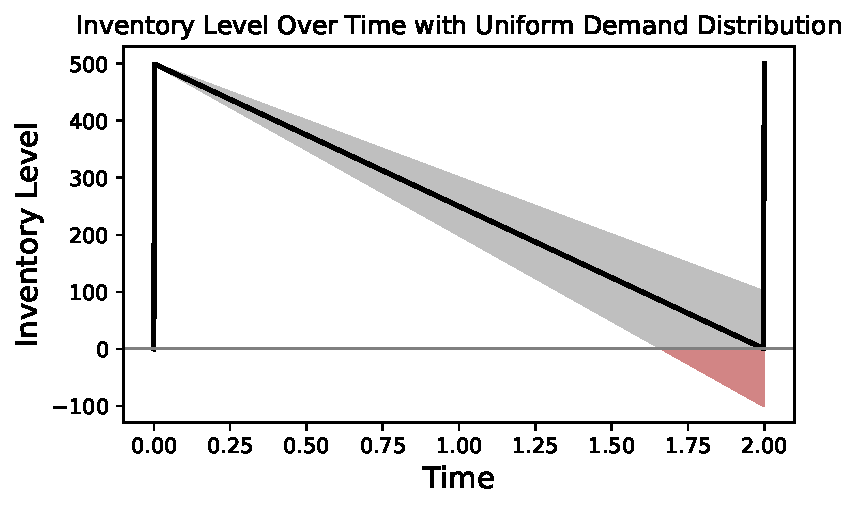
\includegraphics[keepaspectratio]{inventory/safety_files/figure-pdf/cell-2-output-1.pdf}}

\end{example}

よって、発注点 \(r\) は次のように表される。

\[
r = \mu_L + s
\]

従って、\(P(D_L \leq r) = \alpha\) は次のように表される。

\[
P(D_L \leq \mu_L + s) = \alpha
\]

この式を変形すると、

\begin{align}
P(D_L - \mu_L \leq s) &= \alpha \\
P\left(\frac{D_L - \mu_L}{\sigma_L} \leq \frac{s}{\sigma_L}\right) &= \alpha \\
\Phi\left(\frac{s}{\sigma_L}\right) &= \alpha \\
\frac{s}{\sigma_L} &= \Phi^{-1}(\alpha) \\
s &= \sigma_L \Phi^{-1}(\alpha) \\
s &= \sigma \sqrt{L} \Phi^{-1}(\alpha)
\end{align}

ここで、\(\Phi(\cdot)\)
は標準正規分布の累計分布関数であり、\(\Phi^{-1}(\alpha)\)
はその逆関数である。したがって、発注点 \(r\) は次のように表される。

\[
r = \mu_L + s = \mu L + \sigma \sqrt{L} \Phi^{-1}(\alpha)
\]

\(\Phi^{-1}(\alpha)\) は標準正規分布表、Excel、Python
などを用いて求めることができる。

\begin{example}[]\protect\hypertarget{exm-safety}{}\label{exm-safety}

リードタイム \(L = 4\)、平均需要 \(\mu = 100\)、需要の標準偏差
\(\sigma = 20\)、サービスレベル \(\alpha = 0.95\) のとき、発注点 \(r\)
と安全在庫 \(s\) を求める。

リードタイム期間中の平均需要と標準偏差は次のように計算される。

\begin{align}
\mu_L &= \mu L = 100 \cdot 4 = 400 \\
\sigma_L &= \sigma \sqrt{L} = 20 \sqrt{4} = 40 \\
\end{align}

標準正規分布表から \(\Phi^{-1}(0.95) \approx 1.64485\)
を得る。これを用いて安全在庫 \(s\) と発注点 \(r\) を求める。

\textbackslash begin\{align\} s \&= \sigma\_L \Phi\^{}\{-1\}(0.95)
\approx 40 \cdot 1.64485 \approx 65.79 \textbackslash{} r \&= \mu\_L + s
\approx 400 + 65.79 \approx 465.79 \textbackslash end\{align*\}

したがって、発注点 \(r\) は約465.79、必要な安全在庫 \(s\)
は約65.79となる。

Python では、以下のように計算できる。

\begin{Shaded}
\begin{Highlighting}[]
\ImportTok{from}\NormalTok{ scipy.stats }\ImportTok{import}\NormalTok{ norm}

\NormalTok{L }\OperatorTok{=} \DecValTok{4}
\NormalTok{mu }\OperatorTok{=} \DecValTok{100}
\NormalTok{sigma }\OperatorTok{=} \DecValTok{20}
\NormalTok{alpha }\OperatorTok{=} \FloatTok{0.95}

\NormalTok{mu\_L }\OperatorTok{=}\NormalTok{ mu }\OperatorTok{*}\NormalTok{ L}
\NormalTok{sigma\_L }\OperatorTok{=}\NormalTok{ sigma }\OperatorTok{*}\NormalTok{ (L }\OperatorTok{**} \FloatTok{0.5}\NormalTok{)}

\NormalTok{s }\OperatorTok{=}\NormalTok{ sigma\_L }\OperatorTok{*}\NormalTok{ norm.ppf(alpha)}
\NormalTok{r }\OperatorTok{=}\NormalTok{ mu\_L }\OperatorTok{+}\NormalTok{ s}

\BuiltInTok{print}\NormalTok{(}\SpecialStringTok{f"reorder point: }\SpecialCharTok{\{}\NormalTok{r}\SpecialCharTok{:.2f\}}\SpecialStringTok{,  safety stock: }\SpecialCharTok{\{}\NormalTok{s}\SpecialCharTok{:.2f\}}\SpecialStringTok{"}\NormalTok{)}
\end{Highlighting}
\end{Shaded}

\begin{verbatim}
reorder point: 465.79,  safety stock: 65.79
\end{verbatim}

\end{example}

\bookmarksetup{startatroot}

\chapter*{References}\label{references}
\addcontentsline{toc}{chapter}{References}

\markboth{References}{References}

\phantomsection\label{refs}
\begin{CSLReferences}{1}{0}
\bibitem[\citeproctext]{ref-Camm2022-zv}
Camm, Jeffrey, James Cochran, Michael Fry, Jeffrey Ohlmann, David
Anderson, Dennis Sweeney, と Thomas Williams. 2022. \emph{An
introduction to management science: Quantitative approaches to decision
making}. 16th 版. Florence, AL: South-Western College Publishing.

\bibitem[\citeproctext]{ref-Harris1990-gh}
Harris, Ford W. 1990. {「How many parts to make at once」}. \emph{Oper.
Res.} 38 (6): 947--50.

\bibitem[\citeproctext]{ref-Hillier2025-cb}
Hillier, Frederick, と Gerald Lieberman. 2025. \emph{{ISE} introduction
to operations research}. 11th 版. Columbus, OH: McGraw-Hill Education.

\bibitem[\citeproctext]{ref-Scarf1959-xl}
Scarf, Herbert. 1959. {「The optimality of ({S}, s) policies in the
dynamic inventory problem」}.

\bibitem[\citeproctext]{ref-Snyder2019-cy}
Snyder, Lawrence V, と Zuo-Jun Max Shen. 2019. \emph{Fundamentals of
supply chain theory}. 2nd 版. Nashville, TN: John Wiley \& Sons.

\end{CSLReferences}




\end{document}
